% -----------------------------------------------------------------------------
% Trabalhos Relacionados
% -----------------------------------------------------------------------------

\chapter{Granular Materials}
\label{chap:Trabalhos-Relacionados}
    Granular Materials are sets of solid bodies, composed by a given material or different materials. They can have a varied geometries, different densities, friction coefficients, hardness \textit{etc}., but an individual grain must be larger than 100$\mu m$ \cite{Sands_Powders_and_Grains} to ensure the athermous nature. The solid bodies that composes granular materials should be large enough to do not present kinetic fluctuation induced by thermodynamic temperature. Therefore, Brownian motion do not play a role in these systems. Granular materials interact each other when they are in contact, loosing energy by inelastic collision, as well as by friction.

Inelastic collision occurs when two or more grains collide losing part of their initial kinetic energy, in which they have transformed these loss to heat and they may deform in the process \cite{Halliday}. We are modeling the inelastic collision between two grains in section \ref{subsubchap:Reologia}.

\section{Introduction}
\label{subsection:Teoria}

    Examples of granular materials includes sand, stones, soils, drugs, ores, grain foods (rice, corn, soybeans \textit{etc}.), even the asteroid belt and Saturn's rings. The sand alone constitutes 10\% of the materials on surface of planet Earth. Besides that, it is estimated that the second most used material in industries are granular materials, using approximately 10\% of all the energy on the planet, whether in extraction, transport, or processing, with the most used material being water \cite{Sands_Powders_and_Grains}.

    \begin{figure}
        \centering
        \begin{minipage}{.45\linewidth}
            \centering
            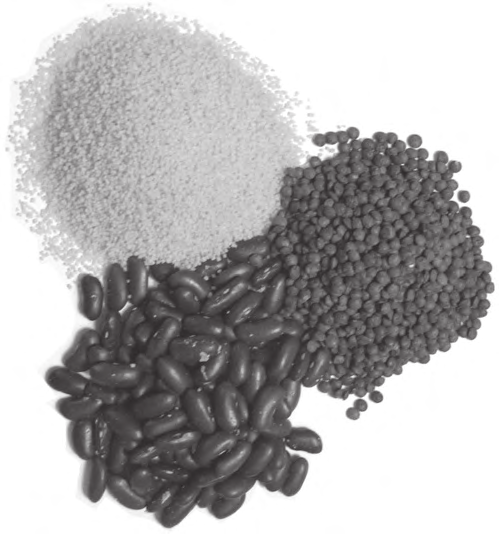
\includegraphics[width=0.9\textwidth]{04-figuras/Exemplo_Alimento.png}
            \subcaption{Grain foods.}
            \label{subfig:exemplo_alimento}
        \end{minipage}
        \begin{minipage}{.45\linewidth}
            \centering
            
\includegraphics[width=0.9\textwidth]{04-figuras/Exemplo_Medicamento.png}
            \subcaption{Drugs.}
            \label{subfig:exemplo_medicamento}
        \end{minipage}
        \begin{minipage}{.275\linewidth}
            \centering
            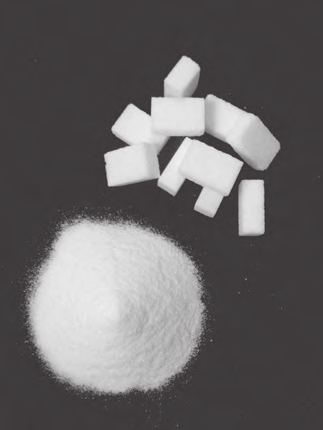
\includegraphics[width=0.9\textwidth]{04-figuras/Exemplo_Acucar.png}
            \subcaption{Sugar.}
            \label{subfig:exemplo_acucar}
        \end{minipage}
        \begin{minipage}{.625\linewidth}
            \centering
            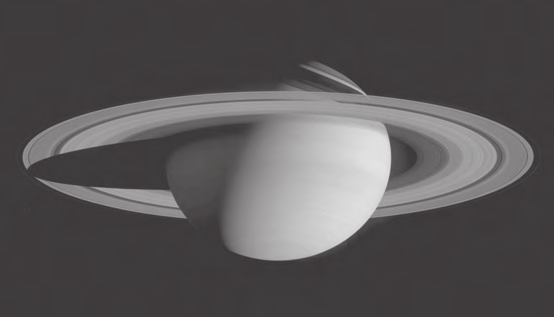
\includegraphics[width=0.9\textwidth]{04-figuras/Exemplo_Saturno.png}
            \subcaption{Saturn and its rings.}
            \label{subfig:exemplo_saturno}
        \end{minipage}
        \caption[Examples of granular materials.]{Examples of granular material. Figures taken from \cite{Granular_Media_Between_Fluid_and_Solid}.}
    \end{figure}

    Due to the absence of Brownian movements, as well as the dissipation of energy in the contacts, granular systems does not undergo spontaneous relaxation of its stable configurations in the absence of external disturbances, and therefore do not present ergodicity. An ergodic system has the characteristic of visit their micro-states of energy spontaneously, implying that their states are all equiprobable when a very long time is taken in account \cite{Unifying_Concepts_in_Granular_Media_and_Glasses, Srdjan-Tese}.

    To demonstrate this non-ergodicity, we can think about a pile of dry sand that rests at a base. If this base does not oscillate, the structure of the pile does not change, and consequently the structure of internal forces will remain unchanged, even if it is heated or cooled in certain limits. This means that sand grains cannot transit between all equipotential states spontaneously, and then this sand pile will rest with internal configurations (chain-forces, stress tensors, grain contact, etc.) unchanged. In the section \ref{subchap:Fenomenologia}, one can find more details.

    Granular materials also have particularities regarding their phases-like, analogously to the state of matter. They are presented individually in solid bodies, and when the grains are close to rest, they constitute the equivalent solid phase. However, if the granular system is slightly agitated, or configured beyond a critical threshold of angle of rest, its behavior can be similar of the liquid. Solid-like and liquid-like granular can coexist and a boundary layer may appear, that indicates the liquid-like flows over the solid-like. When a granular system is vigorously agitated, the behavior is alike gases, they tend to occupy large part of the container which contains them, meaning that its packing fraction ($\phi$) is low and the number of contacts between grains are much rarer, compared to the granular liquid-like and solid-like. An example of the granular states is shown in Figure \ref{fig:exemplo_fases}, where the solid-like phase is in the bottom, the liquid-like phase is flowing through layers in the middle, and the gaseous-like phase is flowing in a higher disordered portion at top. Such classification is still open in the literature, although there are proposals for what would be the granular temperature of the system, in analogy of thermal temperature \cite{Granular_Solids_Liquids_and_Gases}.

    Packing fraction is the measure of the occupied space by the solid portion in relation of the total space occupied by the system. 

    \begin{figure}
        \centering
        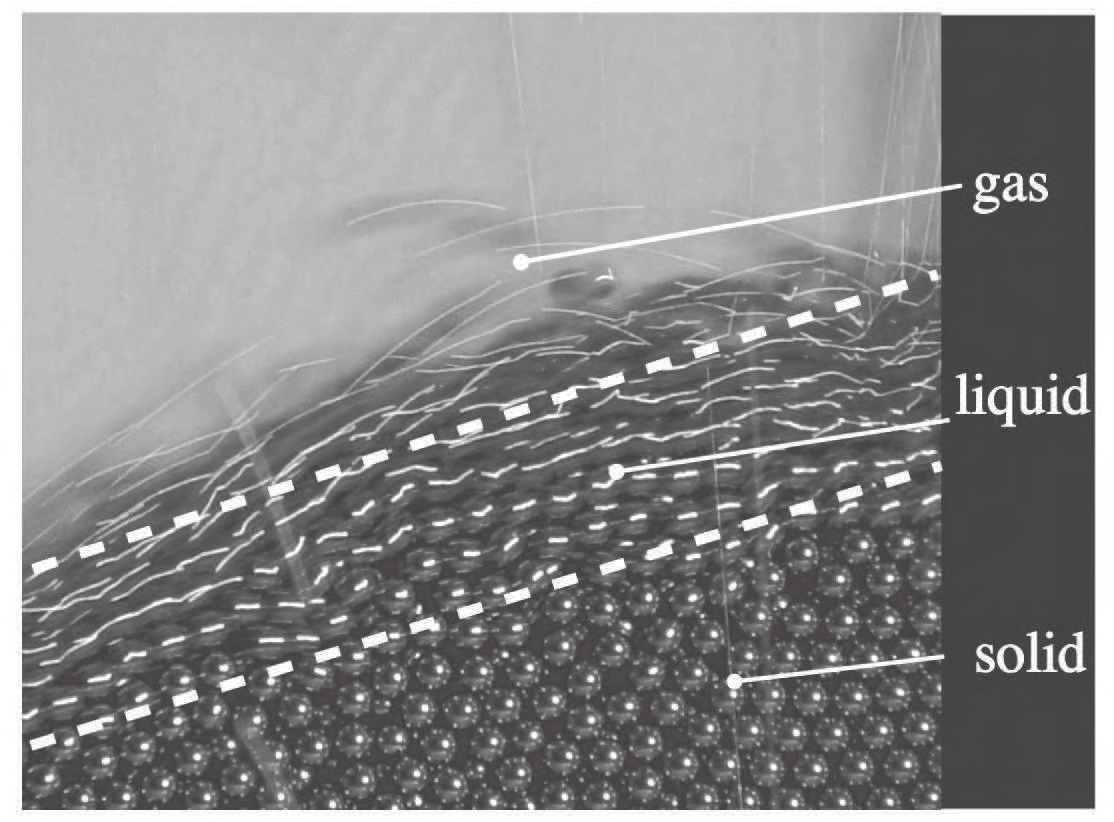
\includegraphics[width=0.9\textwidth]{04-figuras/Exemplo_Fases.png}
        \caption[Granular phases.]{Example of three granular phases according their kinetic energy. Dashed line is a proposition of the phase-like separations. The gas-like, refereed as gas in the Figure, phase is much more agitated and the contact between grains in this region is scarce, compared to the other phases-like. The liquid-like phase, refereed as liquid in the Figure, is moving in layers, and grains are sliding each other. The solid-like phase, refereed as solid in the Figure, is an immobile region that grains are in contact each other and the contact does not change over time. Figure taken from \cite{Granular_Media_Between_Fluid_and_Solid}.}
        \label{fig:exemplo_fases}
    \end{figure}

    A differentiation between granular systems can be a direct result of the interaction forces between grains. Systems that have only repulsive interactions are called dry granules, while wet granules have van der Waals forces in grain-to-grain interactions. In this thesis, we will only consider repulsive contact interactions, although in some cases, there is a fluid surrounding the material. We consider that all the material that is involved by the fluid does not suffer forces of attraction, and therefore, van der Waals force is not included in the interaction between the grains.

\section{Fenomenology}
\label{subchap:Fenomenologia}
    Perhaps the first image related to granular materials remit to the sand pile. In this case, a static pile of sand is heaped on a surface. In a pile like the one shown in Figure \ref{fig:angulo_repouso}, the deposition of the grains forms an angle $\theta _m$ as large as possible, called the angle of movement, and when more material is placed on the pile, the upper layers of the pile run down to the base, restoring the angle to the lowest value $\theta _r$, called the angle of repose \cite{Sands_Powders_and_Grains, Granular_Physics}. The rearrangement of the sand pile after the avalanche can be understood as an example of self-organized criticality in granular materials. A good approximation to the angle of repose is given by:
    \begin{equation}
        \label{equ:atrito}
        \tan(\theta) = \mu _s ,
    \end{equation}
where $\theta$ is the angle of repose, and $\mu _s$ is the coefficient of static friction between grains.

    A system which has no central controller, governed by various agents that interact with rules known in the interaction of agents, and exhibit unforeseen property feature a Complex System. A characteristic property of Complex Systems and granular materials is self-organization. Some authors \cite{Avalanche_Dynamics_in_a_Pile_of_Rice, Avalanche_Prediction_in_a_Self-Organized_Pile_of_Beads, Mixing_and_Segregation_of_Granular_Materials, Measuring_the_flowing_properties_of_powders_and_grains, Revisiting_localized_deformation_in_sand_with_complex_systems, Granular_matter_and_networks, Patterns_and_collective_behavior_in_granular_media, Florent-Tese} classify granular materials within the area of study Complex Systems. An example of self-organization is avalanche\footnote{Avalanche is the process phenomena that dropping some few grains in a pile part of the surface slides.}.

    \begin{figure}
        \centering
        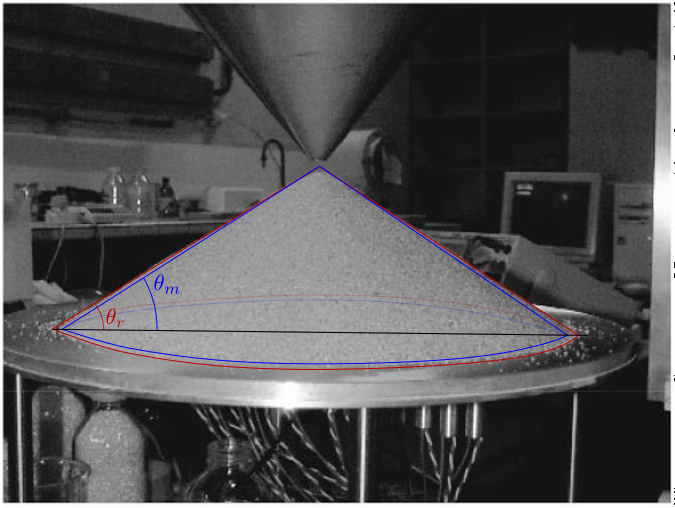
\includegraphics[width=0.9\textwidth]{04-figuras/Sand_Pile_GG_Experiment_Angles.png}
        \caption[Angle of repose and angle of movement.]{Example of angle of repose $\theta _r$ and angle of movement $\theta _m$ in sand. The common values for these angles are $\theta _r = 33^{\circ}$ and $\theta _m = 35^{\circ}$. Figure taken from \cite{Memories_in_Sand}.}
        \label{fig:angulo_repouso}
    \end{figure}

    Also in sand piles, the preparation method of the system is reflected in the angle of repose \cite{Dynamics_at_the_angle_of_repose}. This preparation history allows the system to be configured differently, and therefore, the angle of repose can assume different values using the same material. The angle of repose depends on the relaxation mode in which the pile was made: an inertial mode that relaxation is faster, and a collective mode that relaxation is slower. These dynamics in the angle of repose are called bistability of the angle of repose.

    Another common property of dense granular materials is the force chain, which is the force arrangement through the compressed media. Force chains carry most part of the forces of the media and usually the compression stress coincide with the direction of the force chain \cite{Characterization_of_force_chains_in_granular_material, Granular_and_Complex_Materials}. The number of grains carrying larger forces than the average force decays exponentially with increasing contact force. The force chain is a pathway that the force is transmitted, as shown in Figure \ref{fig:pathway_chain}. The interconnection between two or more branches of force chains forms a force network. The force network is then a subset of the contacts network. The experimental importance of visualizing the chain forces lies in understanding the distribution of the internal forces that sustains the material. As an example, Figure \ref{fig:force_chain} reveals the chain of forces due point force applied on the top of the granular material.

\begin{figure}
    \centering
    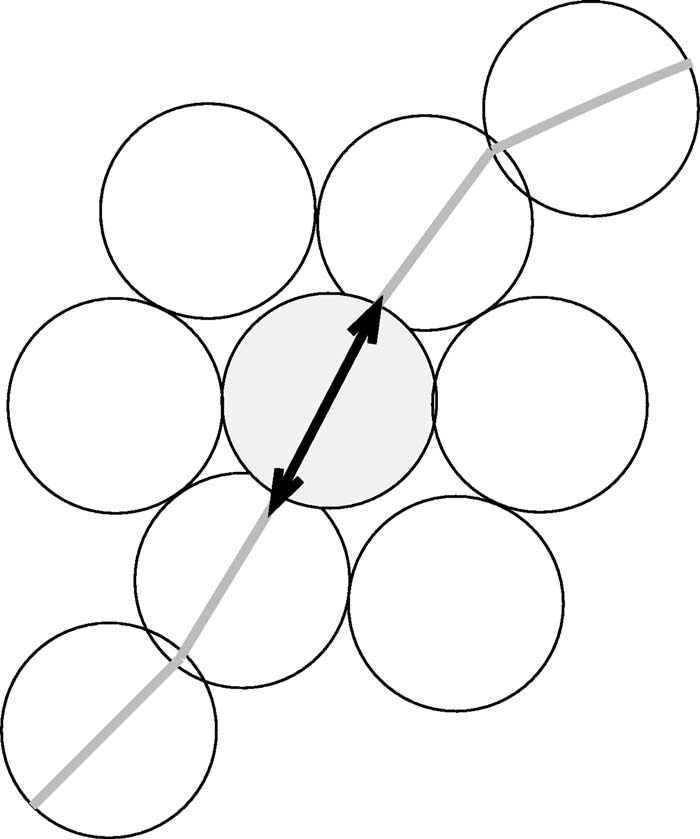
\includegraphics[width=0.25\textwidth]{04-figuras/Force_Chain_Pathway.png}
    \caption[Pahtway of force chain.]{Portion of an idealized force chain. The transmission of the force coincides with the direction of the contacts between grains, forming a path. Figure taken from \cite{Characterization_of_force_chains_in_granular_material}.}
    \label{fig:pathway_chain}
\end{figure}

\begin{figure}
    \centering
    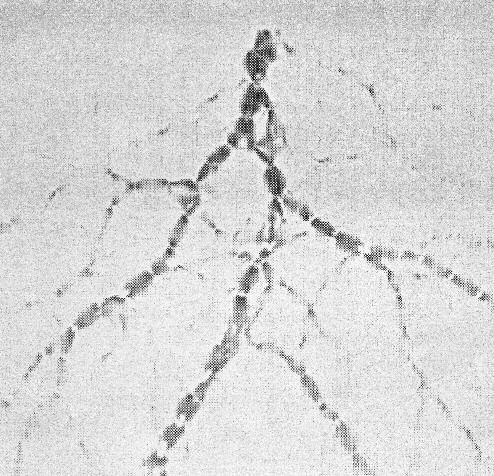
\includegraphics[width=0.5\textwidth]{04-figuras/Cadeia_Forca.png}
    \caption[Example of force chain.]{The application of a point force on top of the material results in the chain of forces, which can be seen in the system's response function, after the gravitational component was subtracted from it. In this case, the system contains photoelastic grains in a two-dimensional space. Photoelastic grains diffracts light differently when a force is applied on it. The force applied on a photoelastic grain produces different tensions, which can be seen by lightning it with a polarized light, and then a polarizing plate blocks the non polarized light. The darker, the greater the stress in the material. Figure taken from \cite{Sensitivity_of_Stress_Response_Function_to_Packing_Preparation}.}
    \label{fig:force_chain}
\end{figure}

    Force chain are important to understand the phenomenon that is present in the arching effect. Arches are collective structures that have mutual support, and, consequently, a chain of forces linking the entire structure, being able to support their own weight and that of all the grains above, preventing them from flowing. In the formation of arches, segregation effects can occur, as verified by Magalhães, C. \cite{Caio-Tese} and the flow regimes in a funnel reported by Magalhães, F. \cite{Felipe-Tese}. Figure \ref{fig:arch_chain} is an example of arch and its chain forces.

\begin{figure}
    \centering
    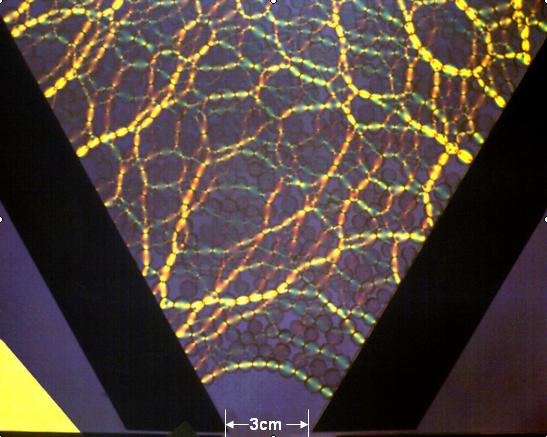
\includegraphics[width=0.5\textwidth]{04-figuras/hopperforcechain.jpg}
    \caption[Arch in a funnel.]{Arch formation in a funnel. Photoelastic grains were used to display the chain forces, and clearly there is a blocking arch with a chain force sustaining all grains above. Figure taken from \cite{Duke_Physics}.}
    \label{fig:arch_chain}
\end{figure}

    To better comprehend the rheology of dense granular materials, there is also the stress tensor, which is a macroscopic quantity of the outer product of contact force between grains and the displacement vector around the analyzed volume \cite{Granular_Physics, Nathalia-Dissertacao, Leticia-Dissertacao, Fabiola-Dissertacao, Force_Chains_Micro_Macro}. The stress tensor in granular materials shows us the preferable direction of a force propagation in the general form, and with it, one can infer how this granular assembly was built \cite{Memories_in_Sand}, like in Figure \ref{fig:pile_stress}.

    An evidence that the preparation history changes the configuration of the material is described in the references \cite{Memories_in_Sand, Sensitivity_of_Stress_Response_Function_to_Packing_Preparation}. The circular base shown in Figure \ref{fig:pile_stress} was made with two different depositions and the pressure profile is measured along the center. In the experiment, the pressure measured at the base varies according to the deposition, with the deposition made from the funnel having a maximum peak pressure around 0.25 and 0.5 of the table radius $r/R$, while in the table deposition made from the sieve presents pressure as a kind of plateau between the center of the table and 0.25 of the radius $r/R$, with the maximum close to the center.

\begin{figure}
    \centering
    \begin{minipage}{.45\linewidth}
        \centering
        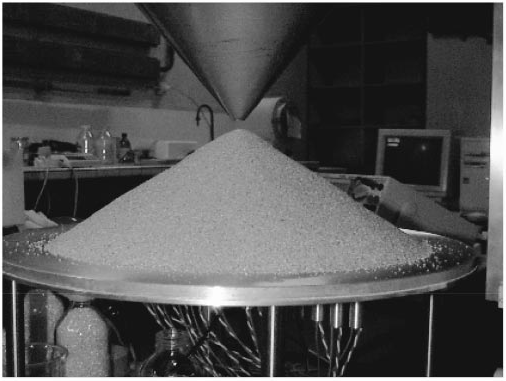
\includegraphics[width=0.9\textwidth]{04-figuras/Sand_Pile_GG_Experiment.png}
        \subcaption{Pile made from a funnel.}
        \label{fig:pressure_pile:GG}
    \end{minipage}
    \begin{minipage}{.45\linewidth}
        \centering
        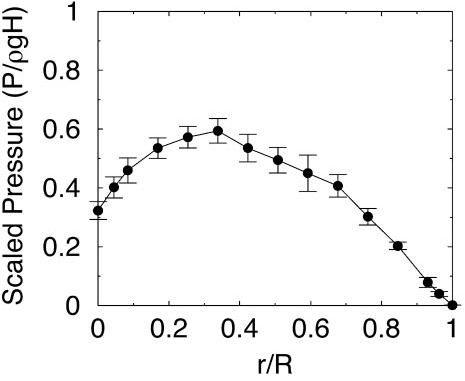
\includegraphics[width=0.9\textwidth]{04-figuras/Sand_Pile_GG_Pressure.png}
        \subcaption{Pressure profile from a funnel.}
        \label{fig:pressure_response:GG}
    \end{minipage}
    \begin{minipage}{.45\linewidth}
        \centering
        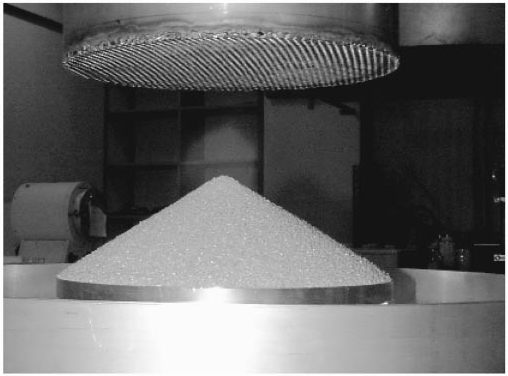
\includegraphics[width=0.9\textwidth]{04-figuras/Sand_Pile_RL_Experiment.png}
        \subcaption{Pile made from a sieve.}
        \label{fig:pressure_pile:RL}
    \end{minipage}
    \begin{minipage}{.45\linewidth}
        \centering
        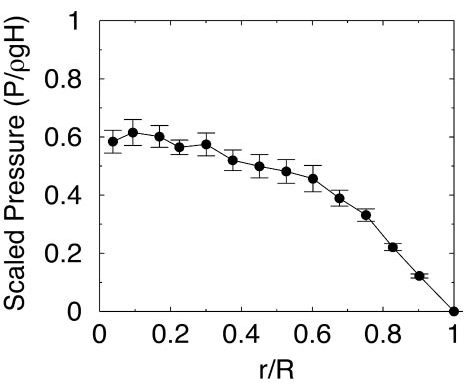
\includegraphics[width=0.9\textwidth]{04-figuras/Sand_Pile_RL_Pressure.png}
        \subcaption{Pressure profile from a sieve.}
        \label{fig:pressure_response:RL}
    \end{minipage}
    \caption[Effect of the preparation history using funnel and sieve.]{The preparation of the sand piles reflects on the pressures measured at the bottom of the pile. In the Panels \ref{fig:pressure_pile:GG} and \ref{fig:pressure_response:GG} the deposition from the funnel creates a pressure profile that peaks outside the center of the pile, while in the Panels \ref{fig:pressure_pile:RL} and \ref{fig:pressure_response:RL} the deposition from the sieve creates a pressure profile that has a plateau and decays on the edges. Figures taken from \cite{Memories_in_Sand}.}
    \label{fig:pile_stress}
\end{figure}    

    A study by Atman \textit{et al.} \cite{Sensitivity_of_Stress_Response_Function_to_Packing_Preparation} shows that different preparation histories of granular materials result in different response functions. As an example, Figure \ref{fig:stress_response} shows two different responses, comparing different geometries of grains: circular and pentagonal. This means that when a localized force is applied over a granular assembly composed by organized assemblies, like the circular grains configuration shown in Panel \ref{fig:stress_response:circle}, the distribution caused by this force, spreads concentrated in two diagonals; while the localized force is applied over a disordered granular assembly, like this pentagonal grains configuration shown in Panel \ref{fig:stress_response:pentagon}, the distribution caused by this force, spreads more uniformly and deeper than the case applied to organized assembly. The response function of this example is the measurement of the stress after applying the load subtracted from the same preparation before applying the load.

\begin{figure}
    \centering
    \begin{minipage}{.45\linewidth}
        \centering
        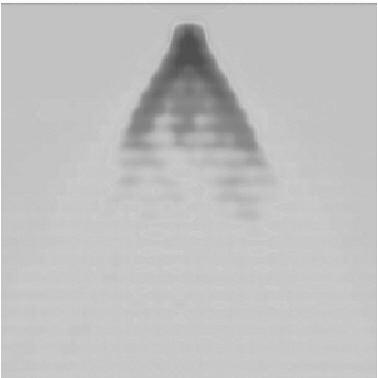
\includegraphics[width=0.9\textwidth]{04-figuras/Funcao_Resposta1.png}
        \subcaption{Circular grains.}
        \label{fig:stress_response:circle}
    \end{minipage}
    \begin{minipage}{.45\linewidth}
        \centering
        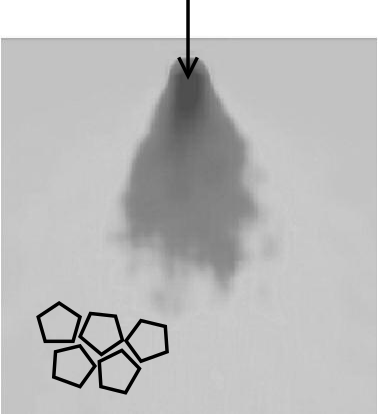
\includegraphics[width=0.9\textwidth]{04-figuras/Funcao_Resposta2.png}
        \subcaption{Pentagonal grains.}
        \label{fig:stress_response:pentagon}
    \end{minipage}
    \caption[Stress response in ordered/disordered granular packings.]{Different granular systems exhibit different response functions. The main difference between these systems is that Panel \ref{fig:stress_response:circle} has higher organization and circular grains, while Panel \ref{fig:stress_response:pentagon} has higher disorder and pentagonal grains. Figures taken from \cite{Sensitivity_of_Stress_Response_Function_to_Packing_Preparation}.}
    \label{fig:stress_response}
\end{figure}

    Response function is the response of a system based on different times of the same system, when an input is applied on this different times, then the difference of the states results in the response of this input \cite{The_Physics_of_Granular_Media}.

    One rich property that many researches studied \cite{Caio-Tese, Felipe-Tese, Eduardo-Tese, Non-Gaussian_behavior_in_jamming_unjamming_transition_in_dense_granular_materials, Da_Cruz-Tese} is the jamming effect. Jamming or clogging, is the effect that dense granular materials suffer when a load is applied and these grains do not move. The consequence is that arch may form to hold the material, as in figure \ref{fig:arch_chain}, but also a cavity may appear if an object is dragged from the inside, like figure \ref{fig:box_Kolb}.

\begin{figure}
    \centering
    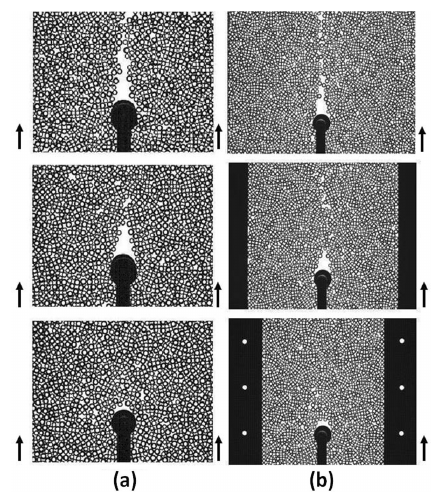
\includegraphics[width=0.5\textwidth]{04-figuras/box_Kolb.png}
    \caption[Cavity formed by a fixed intruder in a dense granular packing.]{The cavity behind the intruder varies according to the packing fraction. The packing fraction is increased in the left panels, from top to bottom as follows: $\phi=$ 0.8050, $\phi=$ 0.8208 and $\phi=$ 0.8262, and they have width equals 13.475 times the intruder diameter. The right panels have packing fraction $\phi=$ 0.8035 and widths, from top to bottom, equals 10.9, 8.5 and 6.9 times the intruder diameter. Figure taken from \cite{Jamming_and_unjamming_by_penetration_of_a_cylindrical_intruder}.}
    \label{fig:box_Kolb}
\end{figure}

    Looking at the scales of granular materials, five separated scales are modeled, according to Radjai \textit{et al.} \cite{Modeling_Granular_Materials}, as shown in Figure \ref{fig:granular_scales}. From now on, when referred to micro-scale, we are talking about dynamics or measures that accounts the effects on contacts or in particles, like rheologycal models of grains and inter-particle forces. Meso-scale are the structure of packing, like chain forces, local packing fraction and coordination number. Coordination number is the number of grains in contact with one single grain. Macroscale is related to the effects on the material and the process, like the stress tensor of the agglomerate and the continuum description of granular materials \cite{Modeling_Granular_Materials}.

\begin{figure}
    \centering
    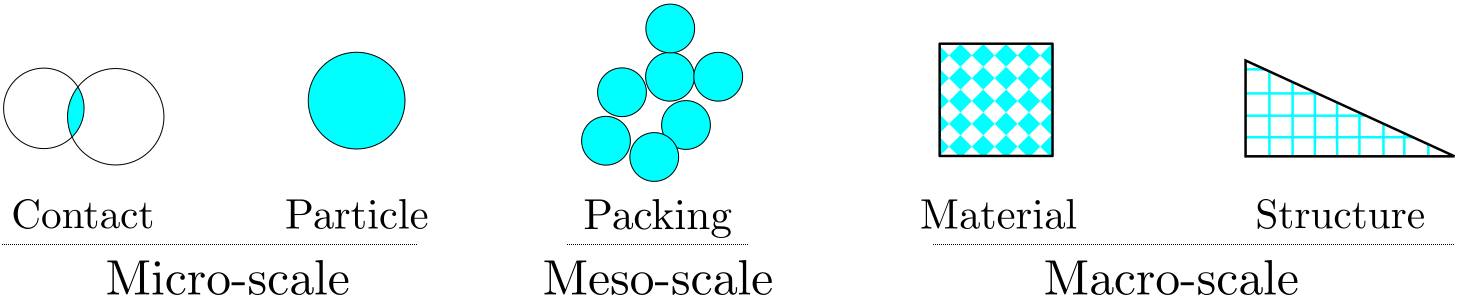
\includegraphics[width=0.99\textwidth]{04-figuras/Granular_Scales.png}
    \caption[Granular scales.]{Scales present in granular measures and effects. The smaller ones are in the contact scale, like contact forces while the higher ones are in landscape scale, like mountains and tectonic formation. Figure adapted from \cite{Modeling_Granular_Materials}.}
    \label{fig:granular_scales}
\end{figure}

    When a wet confined granular material is under pressure, one can see that the liquid shrinks into the material. This phenomena may be contra-intuitive, since when a liquid is squeezed, it is expelled from the container. If the liquid is mixed with granular material, like sand and sea water on a beach, when someone steps on the sand, the surface near the feet becomes dry. This effect was firstly reported by Reynolds \cite{On_the_dilatancy}.

    In the next chapter, we will describe the equations and procedures to carry out simulations of granular materials, taking account the contact model to simulate dry granular systems.
